\section{Native Client Development} % (fold)
\label{sec:native_client_development}
Native Client applications are designed to be cross-platform. To provide cross-platform binaries, the Native Client SDK contains different tool chains - which include different compilers, linkers, assemblers, and other tools to build the application.

\subsection{Toolchains} % (fold)
\label{sub:toolchains}
The tool chains provided by the SDK are:
\begin{itemize}
	\item pnacl: This allows compiling C/C++ code into pnacl bitcode, as described in \ref{sub:portable_native_client} (page \pageref{sub:portable_native_client}). The pnacl toolchain uses the llvm compiler project, and the newlib and libc++ standard library implementations.
	\item nacl-gcc: This allows compiling C/C++ code into verified machine code. NaCl modules can use the newlib or glibc standard C library implementations and libc++ or libstdc++ C++ standard library implementations.
\end{itemize}

\subsubsection{Simplified Building using \lstinline+make+} % (fold)
\label{ssub:building}
The SDK also includes a Makefile called \lstinline+common.mk+ which is used by the included examples and demos to simplify the build process. This makes it easy to write an application for any of the toolchains, without worrying about compiler locations, include file paths, etc.

To specify the compiler, all that needs to be done is to specify the \lstinline+TOOLCHAIN+ environment variable. For example, running \lstinline+make TOOLCHAIN=newlib+ selects the nacl-gcc toolchain and newlib C standard library implementation.

There is also a \lstinline+CONFIG+ environment variable that can be set to specify the compiler's optimisation level. This can be \lstinline+Release+ or \lstinline+Debug+.

To illustrate the usage of \lstinline+common.mk+, listing \ref{getting_started_makefile} shows the Makefile from the SDK's getting started example.

\lstset{language=make,caption={Using the common.mk makefile, as seen in the getting started example},label=getting_started_makefile}
\begin{code}
include $(NACL_SDK_ROOT)/tools/common.mk
TARGET = part2
LIBS = ppapi_cpp ppapi pthread

CFLAGS = -Wall
SOURCES = hello_tutorial.cc

# Build rules generated by macros from common.mk:

$(foreach src,$(SOURCES),$(eval $(call COMPILE_RULE,$(src),$(CFLAGS))))

ifeq ($(CONFIG),Release)
$(eval $(call LINK_RULE,$(TARGET)_unstripped,$(SOURCES),$(LIBS),$(DEPS)))
$(eval $(call STRIP_RULE,$(TARGET),$(TARGET)_unstripped))
else
$(eval $(call LINK_RULE,$(TARGET),$(SOURCES),$(LIBS),$(DEPS)))
endif

$(eval $(call NMF_RULE,$(TARGET),))

\end{code}

Now, running \lstinline+make TOOLCHAIN=newlib CONFIG=Debug+ will compile and build the same sources for the newlib toolchain and Debug config. Running \lstinline+make TOOLCHAIN=all+ compiles and builds the same sources for pnacl, newlib and glibc.

% subsubsection building (end)

\subsubsection{Creating libraries} % (fold)
\label{ssub:creating_libraries}
In C/C++, libraries can be created using the \lstinline+ar+ and \lstinline+ranlib+ tools. This creates a \lstinline+.a+ file which can be later linked with another program. Using the Native Client SDK, this is also supported, but the locations of these tools will depend on the tool chain used.

Thankfully, the common.mk file also provides Makefile macros that make this easy. Using the LIB macro will create the static libraries and also install the libraries into the relevant SDK location. This means it is easy to link in a library for a specific tool chain all using the \lstinline+TOOLCHAIN+ and \lstinline+CONFIG+ variables.

As for dynamic libraries (\lstinline+.so+ files), these are only supported using the glibc tool chain, but \lstinline+common.mk+ takes care of this for us too, by installing the \lstinline+.so+ file if the tool chain is glibc.
% subsubsection creating_libraries (end)

% subsection toolchains (end)

\subsection{Porting existing libraries} % (fold)
\label{sub:naclports}
Many open source C and C++ libraries have been ported to use the Native Client SDK and toolchains. The Native Client team have made a simple platform called naclports to simplify the porting of existing libraries. 

Most of the time, porting an existing library is straight forward, as libraries often have generated makefiles using, for example, a \lstinline+./configure+ script, which allows specifying the required compilers, linkers, etc. needed for building the library. naclports automatically fills in these details. 

Any changes to default build process can be overridden in a script. Any changes to the code of the library can be specified in a patch file, which is applied before the library is built from the original sources.

For example, creating a NaCl port for libpng, an image processing library, is as simple as creating the \lstinline+pkg_info+ file shown in listing \ref{libpng_pkg_info} in naclports. naclports will then automatically download and install the library to the NaCl SDK. Afterwards, the libpng library used normally from any other C/C++ program.

\lstset{language=make,caption={The libpng naclport \lstinline+pkg_info+ file},label=libpng_pkg_info}
\begin{code}
NAME=libpng
VERSION=1.6.8
URL=http://download.sf.net/libpng/libpng-1.6.8.tar.gz
LICENSE=CUSTOM:LICENSE
DEPENDS=(zlib)
SHA1=a6d0be6facada6b4f26c24ffb23eaa2da8df9bd9
\end{code}

% subsection naclports (end)

\subsection{Using the Pepper Plugin API (PPAPI)} % (fold)
\label{sub:using_PPAPI}
\begin{figure}
    \centering
    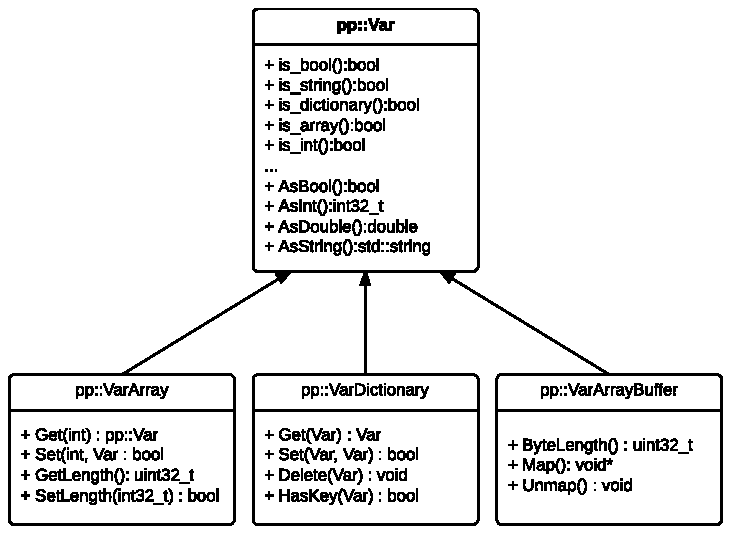
\includegraphics[width=0.8\textwidth]{pp_var-class-diagram.pdf} 
    \caption{A simplified class diagram showing the \lstinline{pp::Var} API}
    \label{fig:pp_var_api}
\end{figure}

To interface with JavaScript, Native Client provides a C and C++ library that allows developers to easily control the browser. One important class that's used in all Native Client modules is the \lstinline{pp::Instance} class, which is initialised when the embed tag is loaded in the HTML page. The class also has the \lstinline{HandleMessage} and \lstinline{PostMessage} functions, which implement message passing between the JavaScript and the C++ module. In JavaScript, JavaScript primitive types as well as reference types can be sent using postMessage. In C++, they are sent and received as \lstinline{pp::Var} objects. Figure \ref{fig:pp_var_api} shows how the \lstinline{pp::Var} classes can be used. 

Notice how C++ types can be extracted using the \lstinline{pp::Var} class. For example, we can extract a C++ \lstinline{double} from the \lstinline{pp::Var} using the \lstinline{pp::Var::AsDouble()} method. Arrays are sent and received as \lstinline{pp::VarArray} objects. JavaScript objects (dictionaries) are sent and received as \lstinline{pp::VarDictionary} objects. Binary data can be sent and received from and to the browser using the \lstinline{pp::VarArrayBuffer} class. The \lstinline{pp::VarArrayBuffer::map()} method returns a pointer to the sent binary data. 

% subsection using_PPAPI (end)

% section native_client_development (end)